\subsection{Hybrid model for wider temperature ranges}

The only restrictive assumption in the derivation of the above model is related to the temperature range of operation.
The linear temperature dependence of rate constants and independence of density (thereby residence time) and void
fraction of the catalyst are valid for a narrow range of temperatures. The other nonlinear effects due to flow-rate and
urea injection are captured in the model. Introducing more complex temperature models for the physical quantities would
lead to parametric models that are not linear (in parameters) and identifiable. Thus, a hybrid model is proposed where
the model structure remains the same while the parameters switch depending on the temperature.

\begin{multline}
        x(k+1) = u_1(k) - \eta(k) \lrb{\frac{u_1(k)}{F(k)}} \lrb{\frac{F(k-1)}{u_1(k-1)}}
                        + \lrb{\frac{u_1(k)}{F(k)}} \pmb \phi^{T}_{NO_x}(k) \pmb \theta^i_{NO_x}
        \\
        T(k), T(k-1) \in \lrb{T_i-\Delta T, T_i + \Delta T}
\end{multline}

Thus, the system switches between models when the current temperature is beyond the $\pm \Delta T$ range of the model.
Experience from the linearized model identification suggests that $\Delta T \approx 25 \, ^0C$ would account for
the changes in system parameters due to drastic changes in temperature.

As the model doesn't have explicit dependence on the unmeasured initial conditions, the parameters for the switched system can be identified by partitioning the data based on the temperature.

\subsubsection{Temperature partitioning}

The temperature partitions work if we have enough data for satisfying PE condition in each of the partitions. From the actual temperature ranges of the test-cell data we get the following narrow partitioning to maximize the length of data available in each of the partitions which can be used for linear temperature model:

\begin{figure}[H]
        \centering
        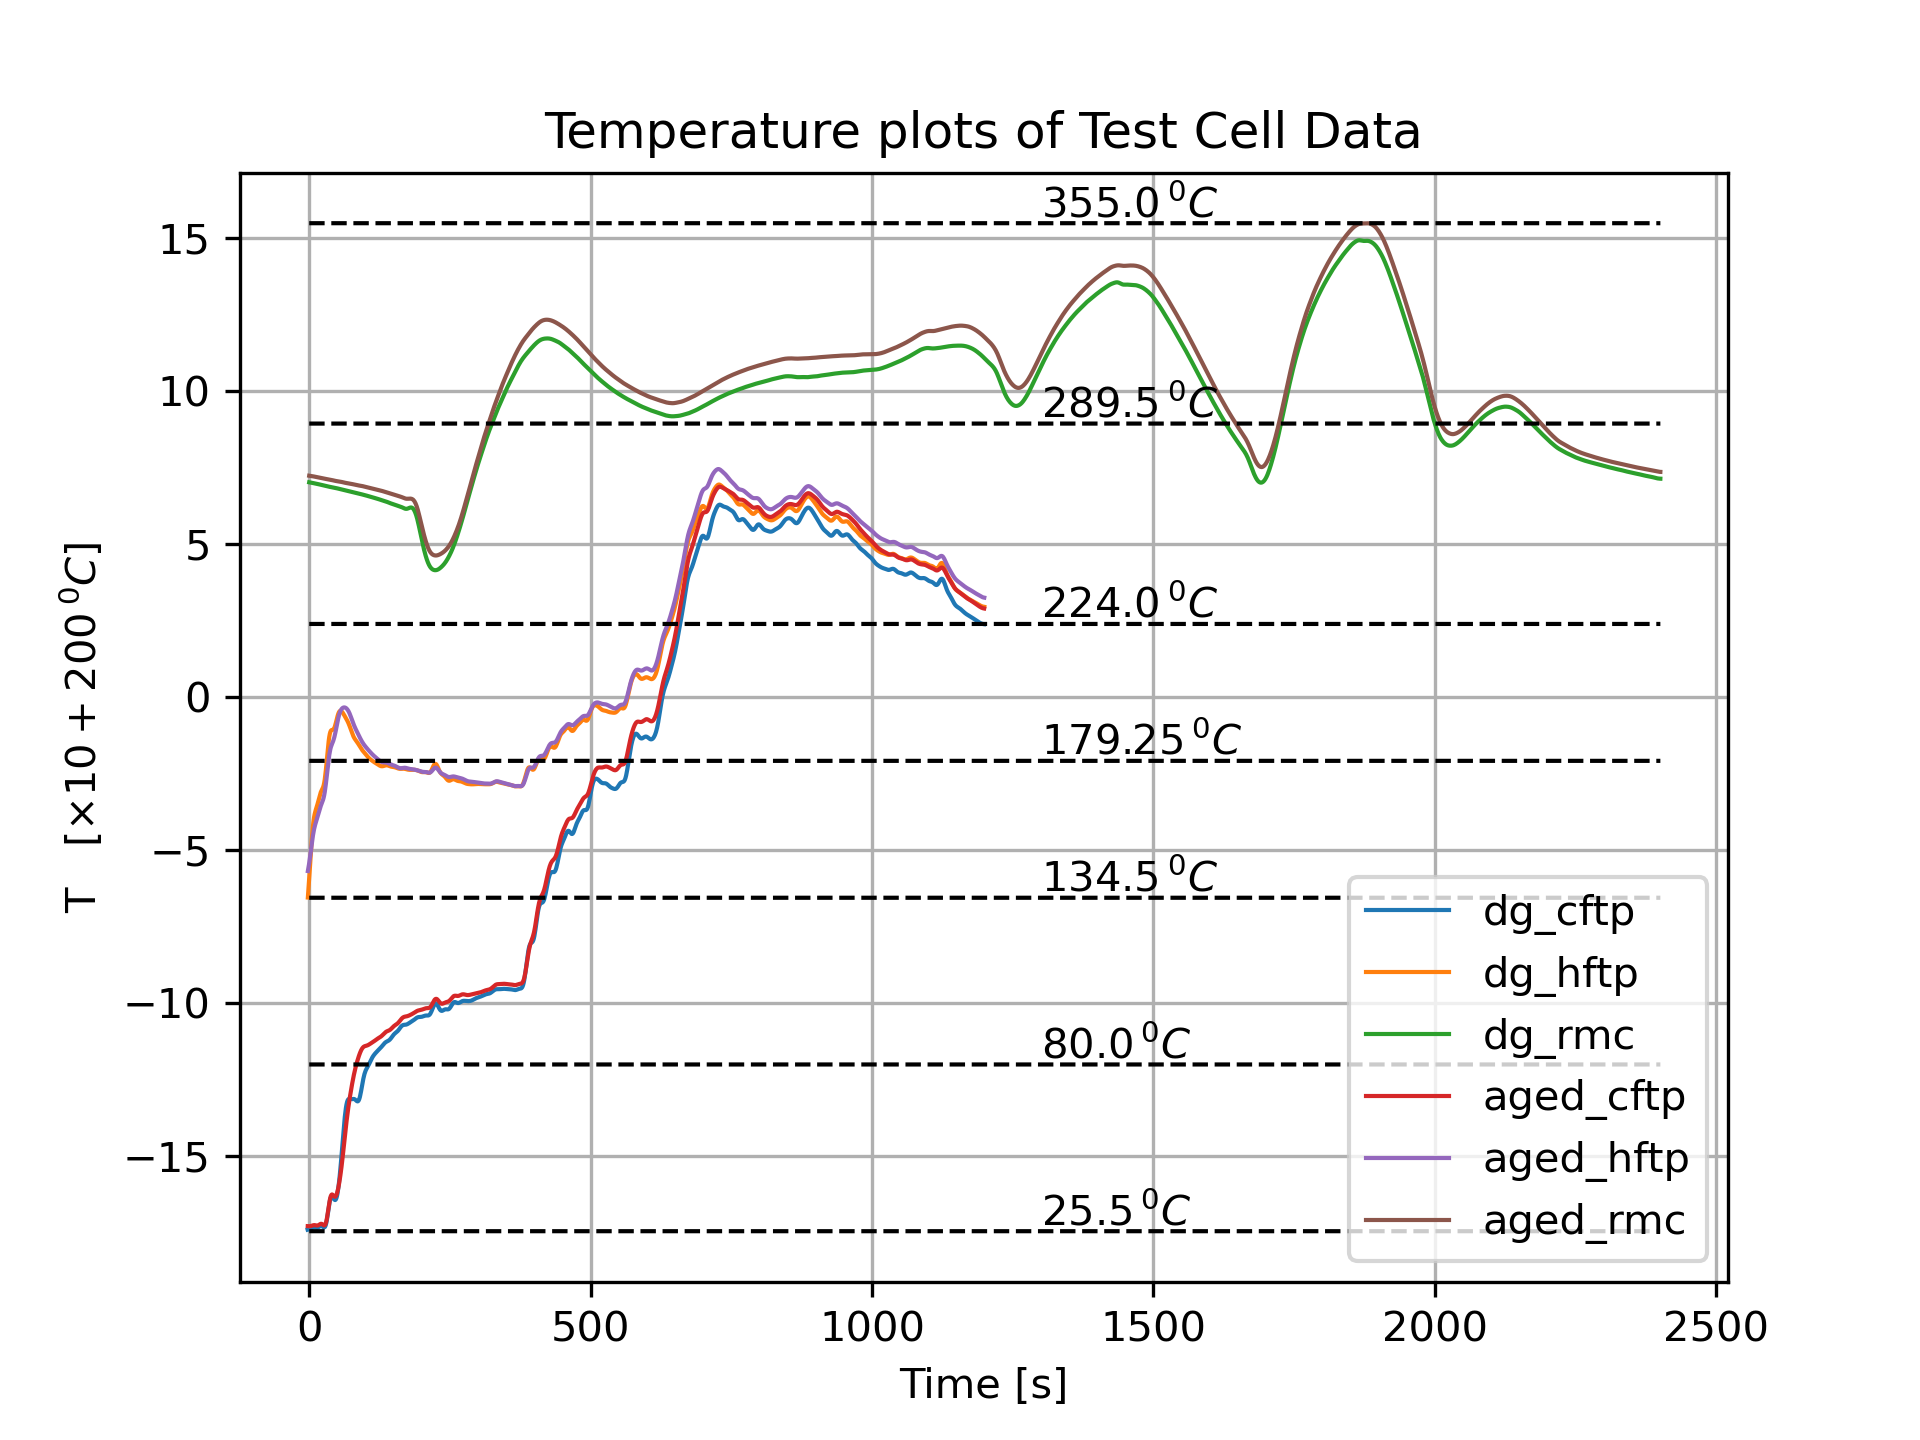
\includegraphics[width = 0.7\textwidth]{\froot/figs/12_figs/hybrid_ssd_T.png}
        \caption{Temperature partitioning for the hybrid model in test-cell case}
\end{figure}

The partitions can be further narrowed if the prediction error is not within the satisfactory range. Alternately, a wider partition, namely high and low temperature zones seems to be enough to consistently model the test-cell data. This partitioning has a high-temperature region where all of RMC test and hot-FTP test lie and a low-temperature region where only a part of the cold-FTP test lies. This partitioning worked the best for the saturated model parameter estimation with quadratic temperature model for $\Gamma k_{ads/scr}$ parametrization. The desaturated model uses the same model with linear temperature model for $k_i, i=ads, scr, od$ parametrization and a quadratic for $\Gamma k_{ads/scr}$ parametrization similar to the saturated system. Further analysis using AVL cruise data is required to obtain the optimal partitioning and order for temperature models of the rate-constants.

\begin{figure}[H]
        \centering
        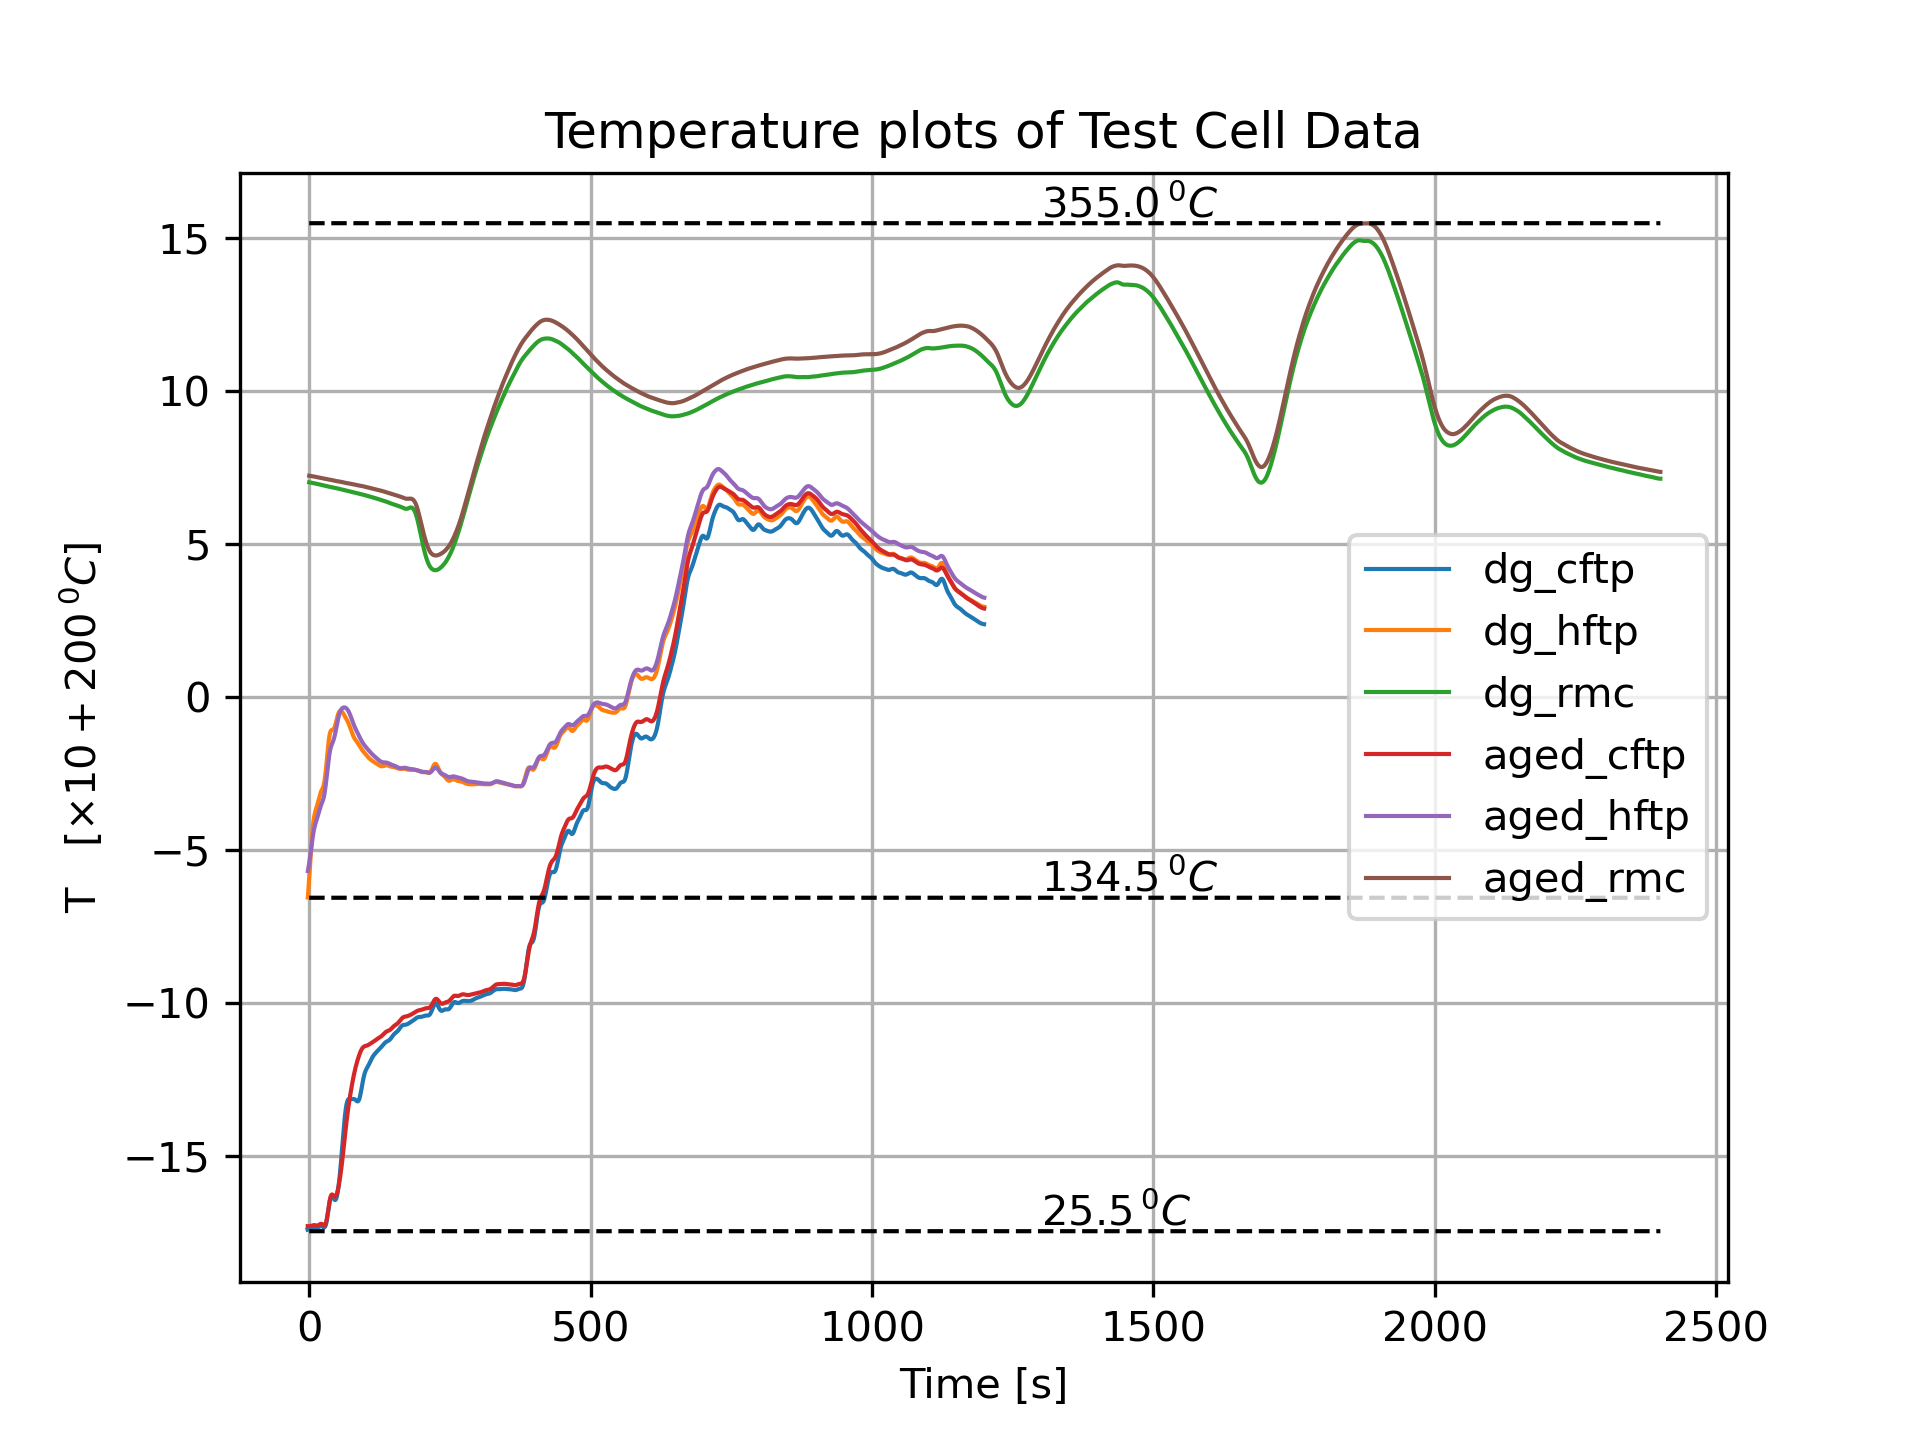
\includegraphics[width = 0.7\textwidth]{\froot/figs/12_figs/hybrid_ssd_hl_T.png}
        \caption{2-zone temperature partitioning for the hybrid model in test-cell case}
\end{figure}
